\documentclass{llncs}
%%\usepackage{verbatim}
%%%% boxed-figure-new.tex
%
% formatting boxed displays

%% some parameters
\newlength{\BFIGURESKIP}
\setlength{\BFIGURESKIP}{3mm}
\newlength{\BFIGURELINEHEIGHT}
\setlength{\BFIGURELINEHEIGHT}{0.3pt}

%% Use the following for a line at the top of a figure,
%% it is raised by \BFIGURESKIP
%% The \par at the end seems to be needed for postscript figures that follow.
\newcommand{\BTOPFIGURELINE}{%
{\rule[\BFIGURESKIP]{\columnwidth}{\BFIGURELINEHEIGHT}}\par%
}

%% A line, with not raised
\newcommand{\BFIGURELINE}{
{\rule{\columnwidth}{\BFIGURELINEHEIGHT}}
% \begin{flushleft}\rule{\columnwidth}{\BFIGURELINEHEIGHT}\end{flushleft}%
}

%% regular figures, the width of the current column of text
\newenvironment{BFIGURE}{
\begin{figure}
\BFIGURELINE
}{%
\par\vskip-\parskip
\BFIGURELINE%
\end{figure}
}

%% regular figures, the width of two column of text, at the top of the page
\newenvironment{BFIGUREDB}{
\begin{figure*}[t!]
}{%
\par\vskip-\parskip
\BFULLFIGURELINE%
\end{figure*}
}

%% figures on a page by themselves
\newenvironment{BFIGUREP}{
\begin{figure}[p!]
\BFIGURELINE
}{%
\par\vskip-\parskip
\BFIGURELINE%
\end{figure}
}

%% figures at the top of the page
\newenvironment{BFIGURET}{
\begin{figure}[t!]
\BFIGURELINE
}{%
\par\vskip-\parskip
\BFIGURELINE%
\end{figure}
}

%% figures at the bottom of the page
\newenvironment{BFIGUREB}{
\begin{figure}[b!]
\BTOPFIGURELINE
}{%
\par\vskip-\parskip
\BFIGURELINE%
\end{figure}
}

%% A line, with not raised
\newcommand{\BFULLFIGURELINE}{
{\rule{\textwidth}{\BFIGURELINEHEIGHT}}
% \begin{flushleft}\rule{\textwidth}{\BFIGURELINEHEIGHT}\end{flushleft}%
}

%% full page figures, the width of the whole page
\newenvironment{BFIGURE*}{
\begin{figure*}
\BFULLFIGURELINE
}{%
\par\vskip-\parskip
\BFULLFIGURELINE%
\end{figure*}
}

%% full page figures, on a page by themselves
\newenvironment{BFIGUREP*}{
\begin{figure*}[p!]
\BFULLFIGURELINE
}{%
\par\vskip-\parskip
\BFULLFIGURELINE%
\end{figure*}
}

%% full page figures, at the top of a page
\newenvironment{BFIGURET*}{
\begin{figure*}[t!]
\BFULLFIGURELINE
}{%
\par\vskip-\parskip
\BFULLFIGURELINE%
\end{figure*}
}

%% another way to do horizontal lines
\newcommand{\UNSPACEFORBOX}{\vspace{-\BFIGURESKIP}}
\newcommand{\HLINE}{\UNSPACEFORBOX\BFIGURELINE\UNSPACEFORBOX}

%% end of boxed-figure-new.tex


\newif\ifpdf
\ifx\pdfoutput\undefined
   \pdffalse     % no PDFLaTeX
\else
  \pdfoutput=1  % PDFLaTeX
   \pdftrue
\fi

\usepackage{alltt}

\ifpdf
\usepackage[pdftex,bookmarks=false,
            plainpages=false,naturalnames=true,
            colorlinks=true,pdfstartview=FitV,
            linkcolor=blue,citecolor=blue,urlcolor=blue]{hyperref}
\else
\usepackage[dvips]{hyperref}
\fi

\ifpdf
\usepackage[pdftex]{graphicx}
\else
\usepackage{graphicx}
\fi

\begin{document}

\pagestyle{empty}

\mainmatter

% --- Author Metadata here ---
%\conferenceinfo{CASSS}{Marseille, France}
%\copyrightyear{2004}
% --- End of Metadata ---

\title{ESC/Java2: Uniting ESC/Java and JML}
\subtitle{Progress and issues in building and using ESC/Java2,
including a case study involving the use of the tool
to verify portions of an Internet voting tally system}

\author{David R.~Cok\inst{1} \and Joseph R.~Kiniry\inst{2}}
\authorrunning{David R.~Cok \and Joseph R.~Kiniry}
\institute{B65 MC01816\\
  Eastman Kodak R \& D Laboratories\\
  Rochester, NY 14650-1816, USA\\
  \email{cok@frontiernet.net}
  \and
  Department of Computer Science, University College Dublin,\\
  Belfield, Dublin 4, Ireland\footnote{Formerly with the
  Security of Systems Group at the 
%  Nijmegen Institute for Computing and Information Science,
  University of Nijmegen.}\\
%   Toernooiveld 1
%   6525 ED Nijmegen, The Netherlands\\
  \email{kiniry@acm.org}}
\date{May 2004}

\maketitle

\newcommand{\myhref}[2]{\ifpdf\href{#1}{#2}\else\htmladdnormallinkfoot{#2}{#1}\fi}

\begin{abstract}
  The ESC/Java tool was a lauded advance in effective static checking
  of realistic Java programs, but has become out-of-date with respect
  to Java and the Java Modeling Language (JML).  The ESC/Java2
  project, whose progress is described in this paper, builds on the
  final release of ESC/Java from DEC/SRC in several ways.  It parses
  all of JML, thus can be used with the growing body of JML-annotated
  Java code; it has additional static checking capabilities; and it
  has been designed, constructed, and documented in such a way as to
  improve the tool's usability to both users and researchers.  It is
  intended that ESC/Java2 be used for further research in, and
  larger-scale case studies of, annotation and verification, and for
  studies in programmer productivity that may result from its
  integration with other tools that work with JML and Java.  The
  initial results of the first major use of ESC/Java2, that of the
  verification of parts of the tally subsystem of the Dutch Internet
  voting system are presented as well.
\end{abstract}

%% \category{D.2.4}{Software Engineering}
%%                 {Software/Program Verification}
%%                 [Formal methods, Programming by Contract]
%% \category{F.3.1}{Logics and Meanings of Programs}
%%                 {Specifying and Verifying and Reasoning about Programs}
%%                 [assertions, invariants, logics of programs,
%%                 pre- and post-conditions, specification techniques]

%% \keywords{JML, ESC/Java, ESC/Java2, static analysis, verification,
%%           annotation languages, program specification} 

% to discuss: specs for JCE packages

\section{Introduction}

The ESC/Java tool developed at DEC/SRC was a pioneering tool in the
application of static program analysis and verification technology to
annotated Java programs~\cite{Flanagan-etal02}.  It was a successor to
the ESC/Modula-3 tool~\cite{ESCModula3}, using many of the same
ideas, but targeting a ``mainstream'' programming language.  ESC/Java 
operates on full Java programs, not on special-purpose languages.  It acts
modularly on each method (as opposed to whole-program analysis), 
keeping the complexity low for industrial-sized programs, but requiring 
annotations on methods that are used by other methods.  The program source
and its specifications are translated into verification conditions; these are passed
to a theorem prover, which in turn either verifies that no problems are found or
generates a counterexample indicating a potential bug. The tool
and its built-in prover operate automatically with reasonable
performance and need only program annotations against which to check
a program's source code.  The annotations needed are easily read,
written and understood by those familiar with Java and are partially
consistent with the syntax and semantics of the separate Java Modeling
Language (JML) project~\cite{jmlpapers,Leavens-etal00}.  Consequently,
the original ESC/Java (hereafter called ESC/Java) was a research
success and was also successfully used by other groups for a variety
of case studies (e.g.,~\cite{Hub03,HOP04}).

% Technically introduce JML and ESC/Java here in more detail. 

Its long-term utility, however, was lessened by a number of factors.
First, as companies were bought and sold and research groups
disbanded, there was no continuing development or support of ESC/Java,
making it less useful as time went by.  As a result of these
marketplace changes, the tool was untouched for over two years and its
source code was not available.

The problem of lack of support was further compounded because its
match to JML was not complete, and JML continued to evolve as research
on the needs of annotations for program checking advanced.  This
unavoidable divergence of specification languages made writing,
verifying, and maintaining specifications of non-trivial APIs
troublesome (as discussed in Section~\ref{sec:usage-exper-date}).

Additionally, JML has grown significantly in popularity.  The
activities of several
groups~\cite{jmlpapers,Burdy-etal03,Leavens-etal00,NimmerErnst01,Bogor03}
generated a number of tools that work with JML.  Thus, many new
research tools worked well with ``modern'' JML, but ESC/Java did not.

Finally, some of the deficiencies of the annotation language used by
ESC/Java reduced the overall usability of the tool.  For example,
frame conditions were not checked, but errors in frame conditions
could cause the prover to reach incorrect conclusions.  Also, the
annotation language lacked the ability to use methods in annotations,
limiting the annotations to statements only about low-level
representations.

The initial positive experience of ESC/Java inspired a vision for an
industrial-strength tool that would also be useful for ongoing
research in annotation and verification.  Thus, when the source code
for ESC/Java was made available, the authors of this paper began the
ESC/Java2 project.

This effort has the following goals:
(1) to make the source consistent with the current version of Java;
(2) to fully parse the current version of JML and Java;
(3) to check as much of the JML annotation language as feasible,
consistent with the original engineering goals of ESC/Java
(usability at the expense of full completeness and soundness);
(4) to package the tool in a way that enables easy application in a
variety of environments, consistent with the licensing provisions of
the source code release; and
(5) as a long-term goal, and if appropriate, to update the related
tools that use the same code base (Calvin, RCC, and
Houdini~\cite{flanagan01houdini}) and to integrate with other
JML-based tools.  This integration will enable testing the tool's
utility in improving programmer productivity on significant bodies of
Java source; the tool will also serve as a basis for research in
unexplored aspects of annotation and static program analysis.
  
We have released over seven alpha versions of ESC/Java2.  The latest
version is available on the \htmladdnormallinkfoot{web}
{http://www.niii.kun.nl/ita/sos/projects/escframe.html} and we
encourage experimentation and feedback.  The source code is available
(and additional contributors are welcome) and is subject to fairly
open licensing provisions.  The discussion below of various features
of JML and ESC/Java2 is necessarily brief; more detail is available in
the implementation notes that are part of an ESC/Java2 release.

The subsequent sections will discuss the most significant changes in creating
ESC/Java2, the extensions to static checking, the backwards
incompatibilities introduced, unresolved semantic issues in JML, and
the direction of the ongoing work in this project.  Also discussed is
ESC/Java2's first serious use: the verification of portions of the
tally subsystem of the Dutch Internet voting system.

Appendices list the details of the enhancements to ESC/Java and those
features of JML that are not yet implemented in ESC/Java2.  We fully
acknowledge that the on-going work described here builds on two
substantial prior efforts: the definition of the Java Modeling Language and
the production of ESC/Java and the Simplify prover in the first place.

\section{JML Example}
The Java Modeling language is described in detail in several other
publications (\cite{Leavens-etal00} and various papers listed at
\cite{jmlpapers}), so here we will give just one example showing some
of the syntax.  The class in Fig.~\ref{fig:example} uses an array to
implement a List.  A few methods with partial specifications are
shown.  They demonstrate the following features of JML:
%\begin{BFIGURE}
%\input{Example.java}
%\caption{A List class with a partial specification.}
%\label{fig:example}
%\end{BFIGURE}
\begin{figure}[htbp]
\begin{verbatim}
//@ model import java.util.List;
//@ model import java.util.ArrayList;
public class Example {
  /*@ spec_public */ private Object[] seq;
                        //@ in list;
                        //@ maps seq[*] \into list;
  //@ invariant seq != null && \elemtype(\typeof(seq)) == \type(Object);

  //@ requires out != null;
  //@ modifies out[*];
  //@ signals (NullPointerException) false;
  //@ ensures seq.length > 0 ==> out[0] == seq[seq.length-1];
  public void reverse(Object[] out) {
    int i = 0;
    int j = seq.length;
    while (i < seq.length) out[i++] = seq[--j];
  }

  //@ public model List list;
  //@ private represents list <- toList(seq);

  /*@ requires input != null;
    @ ensures \result != null;
    @ pure
    @ private model List toList(Object[] input) {
    @   List list = new ArrayList(input.length);
    @   for (int i=0; i<input.length; ++i) list.add(input[i]);
    @   return list;
    @ }
    @*/

  //@ requires i >= 0 && i < length();
  //@ modifies list;
  public void insert(int i, Object o) { seq[i] = o; }

  //@ private normal_behavior
  //@   ensures \result == seq.length;
  //@ pure
  public int length() { return seq.length; }

}
\end{verbatim}
\caption{A List class with a partial specification.}
\label{fig:example}
\end{figure}
\begin{itemize}
\item JML annotations are contained in comments beginning with
\texttt{//@} or \texttt{/*@}.
\item \texttt{model import} statements declare classes imported for
use in annotations.
\item \texttt{spec\_public} indicates that the field named {\em seq}
has public visibility in specifications.
\item The \texttt{invariant} states that after construction {\em seq}
is never null and is an array with \texttt{Object}s as elements.
\item The \texttt{requires} keyword states a precondition for the {\em
reverse} method, namely its argument is presumed to be non-null.
\item The \texttt{modifies} keyword states a frame condition for the
{\em reverse} method, namely that the only fields that are assigned
during its execution are the elements of the \texttt{out} argument.
\item The \texttt{signals} keyword states a postcondition for the {\em
reverse} method that must hold if an exception is thrown, in this case
that it never throws a \texttt{NullPointerException}.
\item The \texttt{ensures} keyword states a postcondition for the {\em
reverse} method that must hold if the method terminates normally.
\item The \texttt{model} declaration declares a public field used in
specifications, typically as an abstract representation of the class.
In this case, the class represents a \texttt{List}.
\item The \texttt{represents} statement indicates the relationship
between the value of the model field and the implementation.
\item The next set of declarations constitute a model method
declaration and its specifications; a model method is only used in
annotations and need not have an implementation.
\item The \texttt{modifies} clause on the {\em insert} method
indicates that it may modify the value of the model field {\em list}
or any field in its {\em datagroup}; the \texttt{in} and \texttt{map}
annotations on the declaration of {\em seq} stipulate that the {\em
seq} field and its array elements are in the {\em list} datagroup.
\item The \texttt{pure} modifier on the {\em length} method indicates
that that method has no side effects (it does not assign to any
fields).
\end{itemize}

This class will compile with javac and will pass all the checks of the
jml checker.  If it is subjected to the ESC/Java2 tool described in
this paper, three warnings are produced, correctly pointing out three
potential problems with this code:
\begin{itemize}
\item The default constructor does not set the value of \texttt{seq}
to a non null array as required by the invariant.
\item The assignment to \texttt{out[i++]} on line 16 is problematic
because the index may be too large for the array; this is fixed by
stating that the length of \texttt{out} must be equal to the length of
\texttt{seq}.
\item An additional warning on that line indicates that the type of
the \texttt{out} array may possibly not allow assignments of Object
references to its elements.
\end{itemize}
\section{Changes to DEC/SRC ESC/Java}

Creating ESC/Java2 required a number of changes to the ESC/Java tool.
Here we present the most significant of these.

\subsection{Java 1.4}

The original work was performed from 1998 to 2000, and Java has
evolved since then.\footnote{In fact, Java 1.5 went beta recently.  No
  work has begun on parsing or statically checking Java 1.5 code.
  Interested parties are welcome to contact the authors with regard to
  this topic.}  The addition required by Java 1.4 is support for the
Java {\tt assert} statement.

JML itself contains a similar assert statement.  Hence, the user may
make a choice between two behaviors.  A Java assert statement may be
interpreted simply as another language feature whose behavior is to be
modeled.  The corresponding behavior is to raise an
\texttt{AssertionError} exception under appropriate circumstances.
Alternatively, a Java assert statement may be interpreted as a JML
assert statement.  In this case, the static checker will report a
warning if the assertion predicate cannot be established.  Both
alternatives are available through user-specified options.

\subsection{Current JML}

The Java Modeling Language is a research project in itself; hence the
JML syntax and semantics are evolving and are somewhat of a moving
target (and there is as yet no complete reference manual).  However,
the core language is reasonably stable.  The following are key
additions that have been implemented; other changes that relate
primarily to parsing and JML updates are listed in the Appendix:

\setlength{\partopsep}{0in}\setlength{\parskip}{0in}\setlength{\itemsep}{0in}\setlength{\topsep}{0in}
\begin{itemize}
\setlength{\partopsep}{0in}\setlength{\parskip}{0in}\setlength{\itemsep}{0in}\setlength{\topsep}{0in}
\item inheritance of annotations and of \texttt{non\_null} modifiers
  that is consistent with the behavioral inheritance of JML;
\item support for datagroups and \texttt{in} and \texttt{maps}
  clauses, which provides a sound framework for reasoning about the
  combination of frame conditions and subtyping;
\item model import statements and model fields, routines, and types,
  which allow abstraction and modularity in writing specifications;
\item enlarging the use and correcting the handling of scope of ghost
  fields, so that the syntactic behavior of annotation fields matches
  that of Java and other JML tools.
\end{itemize}
In addition, all of the differences between JML and ESC/Java noted in
the JML Reference Manual have been resolved.\footnote{The tools still differ 
in (a) the search order for refinement files on the classpath and (b) which
methods may be declared as helper methods.}

\subsection{New verification checks}
Though all of JML is parsed, not all of it is currently checked.
ESC/Java concentrated on checking for possible unexpected exceptions
arising from conditions such as null pointers or out-of-bounds array
indices, since these did not need annotations to be found; annotations
were used, however, to state conditions on method arguments or class
fields that would preclude such errors.  Thus ESC/Java was capable of
checking the pre- and post-conditions of methods as well.  However,
these could only be expressed at a low-level given the limitations of
the ESC/Java input language.

The expanded capabilities of ESC/Java2 allow more thorough checking at
a higher level of abstraction.  This has required only minor changes
in the background axioms used by the theorem prover (mostly regarding
primitive types, though additions to handle the semantics of String
objects are needed).  Most of the changes are implemented by the
appropriate translation of JML features into the theorem prover's
input logic.  The space available in this paper permits only a summary
of the embedding of the above into the underlying ESC/Java
logic\footnote{Subsequent papers are planned that will describe these
  embeddings in more detail.}.

Static checking of the following features has been added to that
performed by ESC/Java.  

% Discuss enrichment of object logic over time to capture more of
% Java and JML's semantics to accomodate functional verification.

\paragraph*{The constraint and initially clauses}
These two clauses are variations on the more common \texttt{invariant}
clause.  They apply to the whole class.  A constraint states a
condition that must hold between the pre-state and the post-state of
every method of a class.  For example,
\begin{center}
\texttt{constraint maxSize == \char'134 old(maxSize); }
\end{center}
states that \texttt{maxSize} is not changed by any method of the
class.  It is implemented by adding the predicate as a postcondition
of every (non-helper) method in the type (and its derived types).

Similarly, \texttt{initially} states a condition that must hold of
every object after construction.  It is implemented by adding its
predicate as a postcondition of every (non-helper) constructor of the
type (but not of its derived types).

\paragraph*{The \texttt{\char'134 not\_modified} expression}
The \texttt{not\_modified} construct is a way of saying, within a
postcondition, that a particular expression has the same value in the
pre-state and the post-state.  That is,
\begin{center}
\texttt{\char'134 not\_modified(x+y) $\equiv$ ( (x+y) == \char'134 old(x+y) )  }.
\end{center}
Uses of the expression in postconditions are expanded inline according
to this definition.

\paragraph*{Checking of datagroups and frame conditions}
JML contains syntax to define 
datagroups~\cite{Leino-Poetzsch-Heffter-Zhou02}.  With datagroups, the items in
an \texttt{assignable} clause may represent sets of program locations,
and those sets may be extended by subtypes.  Each
specification case of a routine may be guarded by a
precondition and may specify the set of store locations that may be
assigned to.

There are a number of cases to be considered in a full implementation.
We will discuss just one here: an assignment statement that has a
left-hand side of \textit{expr.field}.  For this to be a legal
assignment with respect to the specifications, either (a) the
\textit{expr} must evaluate to an object that has been allocated since
the beginning of the execution of the method, or (b) it must be the
case that for every specification case of the method containing the
assignment for which the precondition is true (in the pre-state) there
is at least one store location in the list of assignable locations
that matches \textit{expr.field}.  To match, the field names must be
the same and the \textit{expr} values must evaluate to the same
object.  The matching is complicated by the variety of syntax (e.g.
\textit{expr}\texttt{.*} matches any field of \textit{expr}) and by
the fact that a given field designation may have an accompanying
datagroup and the match may be to any element of the datagroup.
All of this syntax is parsed, and checks are implemented in the logic except
where induction is needed to handle recursive definitions.

Recursive definitions of frame conditions (arising from recursive
structures such as linked lists and trees) are indeed the most
substantial complication in checking datagroups.  As an example,
consider the datagroup of all of the `next' fields of a linked list.
ESC/Java2 currently deals with this by unrolling the recursion to a
fixed depth; since in ESC/Java loops are also unrolled to a fixed
number of iterations, this solution handles common cases of iterating
over recursive structures.

\paragraph*{Annotations containing method and constructor calls}
JML, but not ESC/Java, allows pure method and constructor calls (that
is, methods and constructors without side-effects) to be used in
annotations.  This allows both a degree of abstraction and more
readable and writable specifications.

ESC/Java2 supports the JML syntax and also performs some static
checking.  The underlying prover, Simplify, does support function
definitions and reasoning with functions.  But, as is the rule in
first-order logic, the result of a function in Simplify depends only
on its arguments and not on hidden arguments or on global structures
referenced by the arguments.  Consequently there is a mismatch between
the concept of a pure method in Java and the concept of a function in
the prover.  However, a moderate degree of checking can be performed
without resorting to a full state-based translation and logic if we
(a) identify some methods as functions, where possible, (b) include
the current state of the heap as an additional uninterpreted
parameter, and (c) incorporate the specifications of the called method
as additional axioms.

Dynamic allocations of objects using constructors are simply static
method calls that return new objects and are treated in the same way
as other method calls.  The logic includes axioms that ensure that a
newly allocated object is distinct (reference values are unequal) from
any previously allocated object.  Dynamic allocations of arrays are
translated into first-order logic as functions without difficulty, as
they were in ESC/Java.

\paragraph*{model fields and represents clauses}
The combination of \texttt{represents} clauses and model fields
provides a substantial benefit in abstraction, especially since the
representations may be provided by a subtype \cite{Cheon-etal03}.
Simple representations can be implemented in ESC/Java2 by inlining the
representation wherever the model field is used in an annotation.
However, that proves not to be workable in larger systems.  Instead,
we translate instances of model fields as functions of the object that
owns them and the global state (because model fields can depend upon fields
in other, non-owner, objects).  This allows a useful degree of
reasoning when combined with the class invariants that describe the
behavior of the model fields.

\paragraph*{} The Simplify theorem prover used by both ESC/Java and
ESC/Java2 remains unchanged, except for being compiled for a new
platform (Apple's OS X).  It is written in Modula-3 and consequently
requires compilation for each supported platform.  Although the prover
has definite limitations, as pointed out below, revising it would be a
significant project in its own right.

\subsection{Backwards incompatibilities}
The ESC/Java specification language and JML arose separately; there
was some initial but incomplete work to unify the
two~\cite{Leavens-etal03}.  The ESC/Java2 project intends to have the
tool reflect JML as precisely as reasonable.  In some cases,
discussion about differences resulted in changes to JML.  In a few
cases, some backwards incompatibilities in ESC/Java were introduced.
The principal incompatibilities are these:
\setlength{\partopsep}{0in}\setlength{\parskip}{0in}\setlength{\itemsep}{0in}\setlength{\topsep}{0in}
\begin{itemize}
\setlength{\partopsep}{0in}\setlength{\parskip}{0in}\setlength{\itemsep}{0in}\setlength{\topsep}{0in}
\item The semantics of inheritance of specification clauses and of
  \texttt{non\_null} modifiers was modified to match that defined by
  JML, since the work on JML resulted in an interpretation consistent
  with behavioral subtyping.  JML has a standalone \texttt{also} keyword
that indicates there are inherited explicit or implicit specifications; its
interpretation of specification inheritance is consistent with behavioral
subtyping.  By contrast, ESC/Java's use of inherited specifications had
limitations and was a known source of soundness problems~\cite{Leino-Nelson-Saxe00}.
See
  the section titled ``Inheritance and \texttt{non\_null}'' in the
  ESC/Java2 Implementation Notes for more
  details~\cite{Cok04-Impl-Notes}.
\item The specification \texttt{modifies \char'134 everything} is now
  the default frame axiom.
\item The syntax and semantics of \texttt{initially},
  \texttt{readable\_if} and \texttt{monitored\_by} have changed.
\item ESC/Java2 forbids bodies of (non-model) routines to be present
  in non-Java specification files.
\end{itemize}

\section{Unresolved semantic issues}
%% Gary suggest concentrating on the important issues. - previously pruned

The work on ESC/Java2 has been useful in exposing and resolving
semantic issues in JML.  Since ESC/Java2 is built on a different
source code base than other JML tools, differences of interpretation
in both syntax and semantics arise on occasion.  These are generally
resolved and documented via mailing list discussions\footnote{See
  \texttt{jmlspecs-interest@lists.sourceforge.net},\\
  \texttt{jmlspecs-developers@lists.sourceforge.net}, and \\
  \texttt{jmlspecs-escjava@lists.sourceforge.net} or the corresponding
  archives at \url{http://sourceforge.net/projects/jmlspecs}} by
interested parties.  There are, however, still unresolved issues, most
of which are the subject of ongoing research.
\setlength{\partopsep}{0in}\setlength{\parskip}{0in}\setlength{\itemsep}{0in}\setlength{\topsep}{0in}
\begin{itemize}
\setlength{\partopsep}{0in}\setlength{\parskip}{0in}\setlength{\itemsep}{0in}\setlength{\topsep}{0in}
%% There are "however" in 5 of the 7 sections below. -JRK  - Fixed in earlier revisions
\item \textit{pure routines}: It is convenient and modular to use
  model and Java methods within specifications (model methods are
methods defined for annotations only and not part of the Java source,
such as the {\em toList} method in Fig.~\ref{fig:example}).  The semantics of such
  use is clearer and simpler if such routines are {\em pure}, that is,
  they do not have side-effects.\footnote{Non-pure methods may be used within
annotations in {\em model programs}, which are not discussed in this paper.}
  This is important when evaluating
  annotations during execution, since the checking of specifications
  should not affect the operation of the program being checked.
  Side-effects also complicate static reasoning.  However, some
  side-effects are always present, such as changes to the stack or
  heap or external effects such as the passage of time.  Some are
  often overlooked but can be consequential, such as locking a
  monitor.  Others the programmer may see as innocuous, benevolent
  side-effects, such as maintaining a private cached value or logging
  debugging information in an output file.  An interpretation of the
  combination of purity and benevolent (or ignorable) side-effects
  that is suitable for both static and run-time checking and is
  convenient and intuitive for users is not yet available. (See also
  the discussion of purity checking in~\cite{Leavens-etal03a}.)
\item \textit{exceptions in pure expressions}: The expressions used in
  annotations must not have side-effects, but they may still throw
  exceptions.  In that case the result is ill-defined.  A semantics
  that is suitable for both run-time checking and static verification
  needs to be established.
\item \textit{initialization}: The authors are not aware of any
  published work on specifying the initialization of classes and
  objects in the context of JML; initial work formalizing
  \texttt{\char'134 not\_initialized} was only recently completed for
  the Loop tool.  This task includes providing syntax and semantics
  for Java initialization blocks, JML's \texttt{initializer} and
  \texttt{static\_initializer} keywords, and formalizing the rules
  about order of initialization of classes and object fields in Java.
\item \textit{datagroups}: The \texttt{in} and \texttt{maps} clauses
  and the datagroup syntax are designed to allow the specification of
  frame conditions in a sound way that is extensible by derived
  classes.  We do not yet have experience with the interaction among
  datagroups, the syntax for designating store locations, and either
  reasoning about recursive data structures or checking them at
  run-time.
\item \textit{unbounded arithmetic}: Chalin~\cite{Chalin03} has
  proposed syntax and semantics to enable specifiers to utilize
  unbounded arithmetic in a safe way within annotations.  Tool support
  and experience with these concepts is in progress.  Axioms and proof
  procedures will be needed to support this work in static checkers.
\end{itemize}
There are other outstanding but less significant issues concerning
helper annotations, model programs and the \texttt{weakly},
\texttt{hence\_by}, \texttt{measured\_by}, \texttt{accessible} and
\texttt{callable} clauses.

\section{Usage experience to date}
\label{sec:usage-exper-date}
The SoS group at the University of Nijmegen, along with other members
of the \htmladdnormallinkfoot{European VerifiCard
  Project}{http://www.verificard.org/}, has used ESC/Java for several
projects.  For example, Hubbers, Oostdijk, and Poll have performed
verifications of Smart Card applets using several tools, including
ESC/Java~\cite{HOP04}.  Hubbers has also taken initial steps
integrating several JML-based tools~\cite{Hub03}.

These and other VerifiCard projects relied upon the specifications of
the Java Card 2.1.1 API written and verified by Poll, Meijer, and
others~\cite{MeijerPoll01}.  This specification originally came in two
forms: one ``heavyweight'' specification that used JML models,
heavyweight contract specifications, and refinements, and another
``lightweight'' specification that was meant to be used with ESC/Java
and other verification tools like Jack, Krakatoa, and the Loop
tool~\cite{BergJ01,BurdyRequet02,MarchePaulinMohringUrbain04}.

Writing, verifying, and maintaining these two specifications was a
troublesome experience.  Because of limitations of various tools which
depended upon the specifications, several alternate forms of
specifications were required.  Additionally, it was sometimes the case
that the alternate forms were neither equivalent nor had obvious
logical relationships among them.

This experience was one of the motivators for the SoS group's support
of this work on ESC/Java2.  Now that multiple tools are available that
fully cover the JML language, the incidence of specification reuse is
rising and painful maintenance issues are becoming a thing of the
past.  As a result, early evidence for the success of this transition
is beginning to appear.

\subsection{Transitional Verifications}

First, the specifications of a small case
study~\cite{BreunesseJacobsBerg02} were updated and re-verified by one
of this paper's authors (Kiniry) using ESC/Java2.  The original work
depended upon ``light\-weight'' JML specifications of core Java Card
classes and the verification was performed with ESC/Java and
the Loop tool.  The re-verification effort used the full
``heavyweight'' Java and Java Card specifications and was accomplished
in a single afternoon by an ESC/Java expert.

Second, several members of the SoS group are contributing to updating
the ``heavyweight'' JML specifications of the Java Card API.  As a
part of this work, the Gemplus Electronic Purse case study, which has
been verified partially with ESC/Java~\cite{CatanoHuisman02} and
partially with the Loop tool~\cite{BreunesseJacobsBerg02}, is being
re-verified completely with ESC/Java2 using ``heavyweight''
specifications.

Finally, recent attempts at verifying highly complex Java code
examples written by Jan Bergstra and originally used as stress-tests
for the Loop tool have been encouraging.  Methods that originally took
a significant amount of interactive effort to verify in PVS are now
automatically verified in ESC/Java2, much to the surprise of some of
the Loop tool authors.  This work has caused some re-evaluation of the
balance between interactive and automated theorem proving in the SoS
group.

\subsection{Verification of an Electronic Voting Subsystem}

The first major partial verification using ESC/Java2 took place in
early 2004.

The Dutch Parliament decided in 2003 to construct an Internet-based
remote voting system for use by Dutch expatriates.  The SoS group was
part of an expert review panel for the system and also performed a
black-box network and system security evaluation of this system in
late 2003.  A recommendation of the panel was that a third party
should construct a redundant tally system.  Such a second system would
ensure a double-check of the election count with an independent
system.  It was also thought that such an external implementation
would provide some third-party review of the original work, as the new
implementation would depend entirely upon system design documentation
and data artifacts (e.g. candidate and vote files); no source code
would be shared, or even seen, by the team implementing the redundant
system.

The SoS group bid on the construction of this new system, emphasizing
the fact that they would use formal methods (specifically, JML and
ESC/Java2) to specify, test, and verify the tally system.  The bid was
successful; as a result the SoS group was contracted to write the
tally system.

The most challenging aspect of the contract was \emph{not} the use of
formal methods.  Instead, it was the strict \emph{time requirements}
of the contract, as the system was to be used in the upcoming European
elections.  In particular, the SoS group was asked to construct the
vote counting system (henceforth called the \textsc{KOA} system) in
approximately \emph{four weeks}, with only three developers.

\subsubsection{Development Methodology}

To approach this problem, the three developers (Dr.~Engelbert Hubbers,
Dr.~Martijn Oostdijk, and the second author) partitioned the system
into three subcomponents: file I/O, graphical I/O, and core
data structures and algorithms.  It was decided that, due to the
challenges inherent in full system verification and the restricted
time allotted to the project, while all subsystems would be annotated
with JML, only the third ``core'' subsystem (Dr.~Kiniry's
responsibility) would be fully elaborated in specification.

Additionally, ESC/Java2 would only be used on the core subsystem.  In
the allotted time a ``best-effort'' verification would be attempted, in
addition to all other standard software engineering practices.  This
approach is a standard strategy for lightweight use of formal
methods~\cite{ClarkeWing96}.

\begin{table}[htbp]
  \caption{KOA System Summary}
  \label{tab:KOA_System_Summary}
  \begin{center}
    \begin{tabular}{|l|ccc|}
      \hline
      \quad     & \textbf{File I/O} & \textbf{Graphical I/O} & \textbf{Core} \\
      \hline
       classes & 8                 & 13                     & 6             \\
       methods & 154               & 200                    & 83            \\
      NCSS      & 837               & 1,599                  & 395           \\
      Specs     & 446               & 172                    & 529           \\
      Specs:NCSS & 1:2              & 1:10                   & 5:4           \\
      \hline
    \end{tabular}
  \end{center}
\end{table}

% doublecheck acronym

Table~\ref{tab:KOA_System_Summary} summarizes the size (in
number of classes and methods), complexity (non-comment size of
source, or NCSS for short), and specification coverage of the three
subsystems, as measured with the JavaNCSS tool version 20.40 during
the week of 24 May, 2004.  Assertions were counted by simply counting
the number of uses of appropriate core specification keywords
(requires, ensures, invariant, non\_null, in, set, and modifies).

The size of the code and specifications gives a strong indication of
the complexity of the verification effort.  Longer methods take
significantly more time to specify and verify than short ones.
Classes with many methods, on the other hand, do not necessarily take
much more time to deal with than shorter classes, as effort is coupled
to the complexity of the methods, their specs, and the class
invariants (e.g., many short, simple methods are trivial to verify,
while one long method might take days).

There is very little inheritance in this system.  Visual components
all inherit from a top-level \texttt{Task} class which implements all
state changes in response to external input, and the I/O classes
inherit from an \texttt{AbstractObjectReader}, an Apache licensed
helper class.  Other than that, all classes have no parent (beside
\texttt{Object}).  

Because there is little inheritance and we adopt a closed-system view
on the vote tally system (no classloading is permitted), ESC/Java2's
weak strong support for specifying and reasoning about dynamic binding
is not an issue.

\subsubsection{Specification Coverage and Methodology}

Unsurprisingly, the GUI portion of KOA is the largest subsystem with
the lightest specification coverage, having approximately 1 annotation
for every 10 lines of code.  The focus of the GUI subsystem
specification is a finite state machine that represents the state of
the GUI.  The state of the KOA application is tightly coupled to this
GUI state machine as the vote counting process is highly serialized.

\begin{figure}[htbp]
  \begin{center}
    \ifpdf
    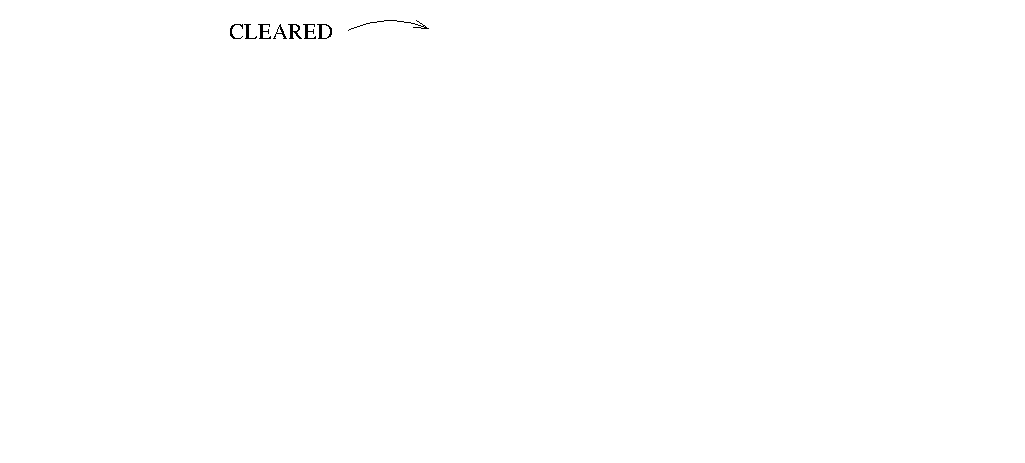
\includegraphics[width=80mm]{koa_state_diagram}
    \else
    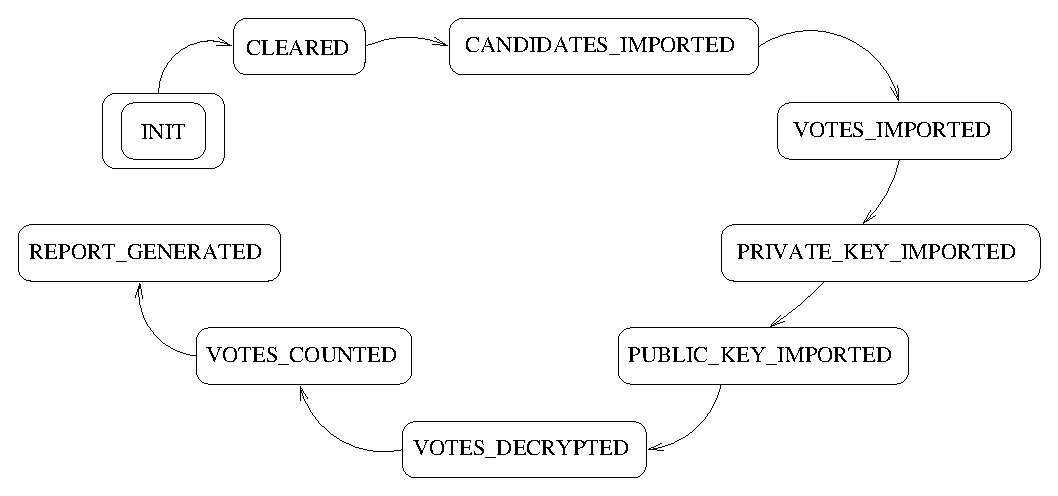
\includegraphics[width=80mm]{koa_state_diagram.eps}
    \fi
    \caption{KOA State Diagram}
    \label{fig:KOA_State_Diagram}
  \end{center}
\end{figure}
Figure~\ref{fig:KOA_State_Diagram} contains a diagram that summarizes
this state machine.  The state of the system is represented in a
(spec\_public) field ``\texttt{state}'' of the main class of the
application.  The state machine is formally modeled using the standard
mechanisms developed in the past by the SoS
Group~\cite{Hubbers_Oostdijk_Poll:2003sec}.

The file I/O subsystem exhibits better specification coverage, much of
which focuses on contracts to ensure that data-structures in the core
subsystem are properly constructed according to the contents of input
files.

The core subsystem understandably has the highest specification
coverage, at over one line of specification for every line of code.
This part of the system was designed by contract, and a small-step
development process was used throughout (i.e., every time a single line
of the specification or the code was changed ESC/Java2 was
re-executed).  Contractual specifications (e.g., requires/ensures-style
and invariants) accounted for the vast majority of the specification;
assertions and invariants were only used to assist the verification
process.

The verification of the key properties of the system, particularly the
property of having a correct tally of votes, are directly tied to the
overall state of the system using invariants of the form
\begin{alltt}
     invariant (state >= <STATE>) ==> (state-field != null);
\end{alltt}
where the states of the system form a total order.  Such an invariant
says that, if the state of the system is at least \texttt{<STATE>},
then the appropriate representation for that state, captured in the
\texttt{state-field}'s datatype is well-formed.  This is a strong
claim because if \texttt{state-field} is non-null, then not only is it
initialized, but all of its invariants hold.

At this time, verification coverage of the core subsystem is good, but
not 100\%.  Approximately 10\% of the core methods (8 methods) are
unverified due to issues with ESC/Java's Simplify theorem prover
(e.g., either the prover does not terminate or terminates abnormally,
as discussed below).  Another 31\% of the core methods (26 methods)
have postconditions that cannot be verified, typically due to
completeness issues discussed above, and 12\% of the methods (10
methods) fail to verify due to invariant issues, most of which are due
to suspected inconsistencies in the specifications of the core Java
class libraries or JML model classes.  The remaining 47\% (39 methods)
of the core verifies completely.

Since 100\% verification coverage was not possible in the timeframe of
the project, and to ensure the KOA application is of the highest
quality level possible, a large number unit tests were generated with
the \emph{jmlunit} tool for all core classes.  A total of nearly 8,000
unit tests were generated, focusing on key values of the various
datatypes and their dependent base types.  These tests cover 100\% of
the core code and are 100\% successful.

\subsubsection{Impressions of ESC/Java2}

ESC/Java2 made a very positive impression on the KOA developers.  Its
increased capabilities as compared to ESC/Java, particularly with
regards to handling the full JML language, the ability to reason with
models and specifications with pure methods, are very impressive.
And, while the tool is still classified as an ``alpha'' release, we
found it to be quite robust (perhaps unsurprising given its history,
the use of JML and ESC/Java2 in and on its own source code, and the
fact that it is passed through seven alpha releases thus far).  But
there are still a number of issues with ESC/Java2 and JML that were
highlighted by the KOA verification effort.

The primary issues that arose include:
\begin{itemize}
\item \emph{String semantics in ESC/Java2 are incomplete.}  In
  particular, one cannot reason effectively about String concatenation
  or equality.  While Java Strings are certainly a non-trivial type,
  they are effectively a pseudo-base type because of their widespread
  use.  Thus, it is vital that this issue be addressed as soon as
  possible.
\item \emph{Issues with reasoning about ``representation-less'' model
    variables.}  If a class declares a model variable but provides no
  statement about how that model relates to the implementation of the
  class (using a \texttt{represents} clause or similar), then
  ESC/Java2 cannot verify assertions that use the model.  We believe
  that a representation-less model variable is equivalent to a ghost
  variable since it is being used as a specification-only variable in
  an API spec.  Thus, by replacing problematic model variables with
  ghost variables in API specifications we can successfully perform
  verifications using the APIs.  This problem indicates either a
  problem with the design and/or use of model variables in JML, or an
  implementation issue with ESC/Java2.
\item \emph{Inconsistencies and ambiguities in the specification of
    core APIs, particularly classes in the \texttt{java.lang} and
    \texttt{java.util} packages and JML model classes.}  This is the
  first large-scale verification effort using ``full'' JML
  specifications of the core JDK.  These ``full'' specifications are
  much more complete and complex than those that were used with
  ESC/Java.  As these core specifications have never been formally
  analyzed for consistency or completeness, it is not surprising that
  the KOA verification effort had problems with their use.  It is
  expected that over time, with more use by a range of JML-compatible
  tools the core specifications will become more consistent and
  complete to the benefit of all JML tool users.
\item \emph{Completeness issues with first-order predicates.}
  First-order predicates are expressed with the \texttt{forall} and
  \texttt{exists} constructs in JML.  Only some of these predicates
  can be used and/or verified in JML-based tools, including ESC/Java2.
  Unfortunately, many of the most interesting invariants in
  non-trivial systems can only be expressed using such constructs.
  Thus, more focus needs to be put on understanding and reasoning
  about such assertions.
\item \emph{Aliasing issues and specification convenience constructs
    for such.}  As usual, reasoning about reference types and avoiding
  aliasing was one of the key issues in verifying the KOA application.
  For example, frequently we wished to say that the elements of a set
  of references were pairwise unequal.  The only way to state this in
  JML today is quite cumbersome, thus the introduction of a new
  specification construct for such seems warranted.
\item \emph{The Simplify prover backend and alternate provers.}
  Simplify is a relatively robust automatic first-order prover,
  especially given its age and the fact that no one has supported it
  in many years.  Unfortunately, Simplify sometimes fails
  catastrophically in one of two ways: it crashes due to an internal
  exception or assertion failure, or it (rarely) consumes as much
  memory as possible and halts.  Neither of these situations is
  reasonable, of course, but as there is no support for Simplify, the
  problems indicated by these affects are rarely correctable.  It is
  our intention to initially augment, then eventually replace,
  Simplify with an alternative modern, supported prover.
\end{itemize}

% JML test runs: 18/19 (meaningful/total)
% JML test runs: 35/6716 (meaningful/total)
% JML test runs: 20/37 (meaningful/total)
% JML test runs: 36/64 (meaningful/total)
% JML test runs: 48/210 (meaningful/total)
% JML test runs: 97/776 (meaningful/total)
% (+ 19 6716 37 64 210 776)

\section{Ongoing work}
The work on ESC/Java2 is continuing on a number of fronts.

\paragraph*{Language Issues} Two obvious and related ongoing tasks are
the completion of additional features of JML, accompanied in some
cases by additional research to clarify the semantics and usability of
outstanding features of JML.  Usage of JML is now broad enough that an
accompanying formal reference document would be valuable.  As
tools such as ESC/Java2 become more widely used, users will also
appreciate attention to performance, to the clarity of errors and
warnings, and to the overall user experience such tools provide.

\paragraph*{Case Studies} The current implementation supports the
static checking of a stable core of JML.  With this initial
implementation of frame condition checking, of model fields,
represents clauses and use of routine calls in annotations, ESC/Java2
can now be used on complex and abstract specifications of larger
bodies of software.  Consequently, there is a considerable need for
good experimental usage studies that confirm that this core of JML is
useful in annotations, and that the operation of ESC/Java2 (and
Simplify) on that core is correct and valuable.

\paragraph*{Verification Logic} The logic into which Java and JML are
embedded in both ESC/Java and ESC/Java2, by design and admission of
the original authors, neither identifies all potential errors (e.g.,
because not all aspects of Java are modeled in the logic) nor avoids
all false alarms (e.g., because of limitations in the prover).  This
was the result of an engineering judgment in favor of performance and
usability.  Research studying expanded and larger use cases may show
whether this design decision is generally useful in practical static
checking or whether a fuller and more complicated state-based logic is
required for significant results to be obtained.

A related issue is the balance between automated and manual proof
construction.  Use of verification logics will likely be limited to
narrow specialties as long as proof construction is a major component
of the overall programming task.  Thus, automation is essential,
though it is expected that full automation is infeasible.  The degree
of automation achievable will continue to be a research question.
However, we believe that broad adoption of automated tools for program
checking will require that users only need interact at high levels of
proof construction.

\paragraph*{User Feedback} The purpose of using theorem provers for
static analysis, runtime assertion checking, or model checking is to
find errors and thereby improve the correctness of the resulting
software.  Thus, the orientation of a tool must be towards effectively
finding \emph{and interpreting} examples of incorrect behavior.  A
complaint (e.g.,~\cite{GroceVisser03}) in using such technologies is
that it is difficult to determine a root cause from the counterexample
information provided by the tool, whether it is a failed proof or an
invalid test or execution history.  The ESC/Java project implemented
some work towards appropriately pruning and interpreting
counterexample and trace
information~\cite{LeinoMillsteinSaxe:ErrorTraces}, but there remains
room for improvement.  Machine reading of the Simplify output coupled
with other tools is also a means to easier
interpretation~\cite{csallner05check}.

\paragraph*{Tool Integration} Finally, though not part of this specific
project, an integration of tools that support JML would be beneficial
for programmer productivity.  A productive programmer's working
environment for a large-scale project that uses these tools would need
them to be integrated in a way that they seamlessly communicate
with one another.  A programmer using the tools would naturally move
among the various tasks of designing, writing, testing, annotating,
verifying and debugging, all the while reading, writing and checking
specifications.  Design, specifications and code might all be built up
incrementally.  Thus, the tools would need to be integrated in a way
that allows efficient and iterative behavior.

\section{Conclusion}

The progress and case studies described above have shown that
ESC/Java2 is ready for serious evaluation and use, even in its early
``alpha'' releases.  Our ability to verify large portions of a
critical, public system in a very short time frame is a strong
statement about the state of the tool and the underlying theory of
extended static checking.

Additional evidence comes from several groups around the world that
are using ESC/Java2 for instruction and research.  We are aware of
over a half dozen groups that are using ESC/Java2 for new research in
verification, and nearly ten courses are using it for instruction in
software engineering, verification, pedagogical instruction of Java,
and grading.  We continue to see growing interest in ESC/Java2,
verification, and extended static checking in general.

One can observe this work in tool creation and evaluation from a
number of perspectives.  Certainly such work creates working
prototypes that test in practice theories of programming and
specification language semantics.  It also exercises and validates
ideas in automated logical reasoning.  We prefer to use the viewpoint
of programming productivity, particularly given the industrial working
environment of the first author.  In that context we observe the
existence and general use across multiple research groups of the
combination of various tools that support using JML with Java
programs; this suggests to us that the syntax and semantics of the
core of JML are sufficiently useful and natural to provide a basis for
future wider use.  With respect to logical reasoning, a useful degree
of automation is achievable in at least some aspects of static
checking tasks; removing the details of proof construction from a
programmer's tasks is essential to larger scale acceptance of such
tools.

However, the surrounding issues are as relevant to programmer
acceptance and productivity.  Tools must have intuitive and
unsurprising behavior. They must be efficient in elapsed run-time, but
also in the time needed to interpret and act upon the results.  They
must integrate well with other tools of the same family and with
commonly used programmer's working environments.

%%TODO - Gary doesn't like the second part of the following paragraph

There is progress on enough of the above vectors that one might well
be optimistic about the eventual success of the enterprise as a whole.
After all, the goal need not be fully automated verification of an
arbitrary computer program.  Reflect that a computer-produced proof of
a mathematical conjecture that cannot be understood at least in its
broad outlines by mathematicians leaves those mathematicians
unsatisfied and unsettled with respect to the proof.  Similarly, we
expect that ``verifications'' of programs whose overall design is
incomprehensible to readers of the program (not to mention its author)
will not engender much confidence in the verification.  If programming is
writing for others and we expect that the authors could explain their
programs to their colleagues, we may well have a chance at being able
to explain those programs to a computer.


%ACKNOWLEDGMENTS are optional
\section{Acknowledgments}
The authors would like to acknowledge both the work of the team that
developed ESC/Java as well as Gary Leavens and collaborators at Iowa
State University who developed JML.  In addition, Leavens and students
engaged in and helped resolve syntactic and semantic issues in JML
raised by the work on ESC/Java2.  These teams provided the twin
foundations on which the current work is built.  Other research groups
that use and critique both JML and ESC/Java2 have provided a research
environment in which the work described here is useful.  Thanks are
due also to Leavens for his comments on an early draft of this paper.

Joseph Kiniry is supported by the NWO Pionier research project on
Program Security and Correctness and the VerifiCard research project.

%
% The following two commands are all you need in the
% initial runs of your .tex file to
% produce the bibliography for the citations in your paper.
\bibliographystyle{abbrv}
\bibliography{abbrev,PASTE2004,CASSIS2004}
% To create the self-contained file - comment out the line above and include the
% contents of the .bbl file here
%% \begin{thebibliography}
%% \end{thebibliography}

% You must have a proper ".bib" file
%  and remember to run:
% latex bibtex latex latex
% to resolve all references
%
% ACM needs 'a single self-contained file'!
%
%APPENDICES are optional

%\balancecolumns

\appendix

\section{Principal changes to ESC/Java}
\setlength{\partopsep}{0in}\setlength{\parskip}{0in}\setlength{\itemsep}{0in}\setlength{\topsep}{0in}
\begin{itemize}
\setlength{\partopsep}{0in}\setlength{\parskip}{0in}\setlength{\itemsep}{0in}\setlength{\topsep}{0in}
\item[] \textit{Language semantics}
\item inheritance of annotations and of \texttt{non\_null} modifiers
  that is consistent with the behavioral inheritance of JML;
\item support for datagroups and \texttt{in} and \texttt{maps}
  clauses, which provides a sound framework for reasoning about the
  combination of frame conditions and subtyping;
\item model import statements and model fields, routines, and types,
  which allow abstraction and modularity in writing specifications;
\item enlarging the use and correcting the handling of scope of ghost
  fields, so that the syntactic behavior of annotation fields matches
  that of Java and other JML tools;
\item[]
\item[] \textit{Language parsing}
\item parsing of all of current JML, even if the constructs are
  ignored with respect to typechecking or verification;
\item support for refinement files, which allow specifications to be
  supplied in files separate from the source code or in the absence of
  source code;
\item heavyweight annotations, which allow some degree of modularity
  and nesting;
\item auto model import of the \texttt{org.jmlspecs.lang} package,
  similar to Java's auto import of \texttt{java.lang};
\item generalizing the use of \texttt{\char'134 old}, \texttt{set}
  statements and local ghost variables, to provide more flexibility in
  writing specifications;
\item introduction of the \texttt{constraint}, \texttt{represents},
  \texttt{field}, \texttt{method}, \texttt{constructor},
  \texttt{\char'134 not\_modified}, \texttt{instance}, \texttt{old},
  \texttt{forall}, \texttt{pure} keywords as defined in JML;
\item consistency in the format of annotations in order to match the
  language handled by other JML tools;
\item equivalence of \texttt{\char'134 TYPE} and \texttt{java.lang.Class};
\item a beginning of a semantics for String objects, namely the
  freshness of the result of built-in + and equality and inequality of
  String literals.
\end{itemize}
In addition, all of the differences between JML and ESC/Java noted in
the JML Reference Manual have been resolved.

\section{Aspects of JML not yet\\implemented in ESC/Java2}

Though the core is well-supported, there are several features of JML
which are parsed and ignored, some of them experimental or not yet
endowed with a clear semantics, and some in the process of being
implemented.  For those interested in the details of JML and
ESC/Java2, the features that are currently ignored are the following:
\setlength{\partopsep}{0in}\setlength{\parskip}{0in}\setlength{\itemsep}{0in}\setlength{\topsep}{0in}
\begin{itemize}
\setlength{\partopsep}{0in}\setlength{\parskip}{0in}\setlength{\itemsep}{0in}\setlength{\topsep}{0in}
\item checking of access modifiers on annotations and of the
 \texttt{strictfp}, \texttt{volatile},
  \texttt{transient} and \texttt{weakly} modifiers;
\item the clauses \texttt{diverges}, \texttt{hence\_by},
  \texttt{code\_contract}, \texttt{when}, and \texttt{measured\_by};
\item the annotations within \texttt{implies\_that} and {\tt
    for\_example} sections;
\item some of the semantics associated with the initialization steps prior to
  construction;
\item multi-threading support beyond that already provided in ESC/Java;
\item serialization;
\item annotations regarding space and time consumption;
\item full support of recursive \texttt{maps} declarations;
\item model programs;
\item some aspects of store-ref expressions;
\item verification of anonymous and block-level classes;
\item verification of set comprehension and some forms of quantified
  expressions;
\item implementation of \texttt{modifies \char'134 everything} within
  the body of routines.
\end{itemize}


% That's all folks!
\end{document}

      From:     Marieke.Huisman@sophia.inria.fr
      Subject:        Re: Reminder: deadline submissions for Cassis is approaching 
      Date:   21 July, 2004 11:37:28 CDT
      To:       kiniry@acm.org
      Cc:       cassis04@belle.inria.fr

Dear Joe,

We are pleased to inform you that your paper

  ESC/Java2: Uniting ESC/Java and JML

has been accepted to appear in the proceedings of Cassis 2004.
All papers have been carefully reviewed by at least three reviewers. 
Please follow closely their suggestions for the final version of your 
paper.

Please send us your camera-ready manuscript by September 17, 2004. We 
ask you to follow precisely Springer's formatting guidelines for the 
LNCS series (available at http://www.springer.de/comp/lncs/authors.htm
l) and to send the LaTeX sources, the final ps and pdf in due time to 
cassis04@sophia.inria.fr.

The reviews and comments are attached below.  Again, do your best to 
follow the advice in revising your paper.

Congratulations on your fine work.  If you have any additional 
questions, please feel free to get in touch.

Best regards,

The Cassis organisers

Gilles Barthe
Lilian Burdy
Marieke Huisman
Jean-Louis Lanet
Traian Muntean

Review 1
========

Title:  ESC/Java2: Uniting ESC/Java and JML
Author: David Cok and Joseph Kiniry



Overall opinion: Strong Accept/Weak Accept/Weak Reject/Strong Reject


Weak Accept

Confidencen: Expert/Average/Low


Expert

Summary of the paper


This is a status report on the ESC/Java2 tool, and the progress in 
enhancing
it to fit in with full JML (Java Modelling Language).

General comments

This a a good description of what has been done to ESC/Java2, and some
of the problems that have arisen as it has been extended to handle 
full JML
and solutions to those problems.   It then describes an impressive 
case
study
in which ESC/Java2 was used, with some successes but also some 
problems.
There are two main problems with the paper currently, which need to be
addressed before it is published for wider reading than CASSIS:

1.  A lot of JML concepts and terminology are used without
explanation.  For many readers, this will be a problem.  So a short
introduction (1 page max) should be added, giving an example of a
very small JML class spec, and introducing the terminology: ensures,
requires, invariant, model, datagroups, represents etc.

Example added.

2. Some of the descriptions of the problems that came up, and
(especially) the solutions that were taken, are too terse or
missing.  A little more detail is needed in places like:

Last sentence of Sect 2.2 says "virtually all of the diffs betwee
JML and ...  have been resolved."  -- explain which ones have not,
or at least say how many have not and why.

A footnote was added to list the two (known) minor differences.

p4: The discussion of expr.* locations is interesting -- you leave
it unclear how much of this is currently supported.

Clarified.

p4: "Annotations containing routine calls and dynamic allocations"
These seem to be two separate topics, so could be discussed
separately.  The two sentences about dynamic allocations are
unclear, so need rewriting.

Revised and expanded a bit.

p5: "This also changed the usage and semantics of the also keyword."
Explain!

Explained and references added.

Detailed comments

p4: "Consequently there is [still] a mismatch between the concept of
a [pure?]  method in Java and the concept of a function in the
prover."  (It was unclear if you are talking of arbitrary Java
methods, or just the pure ones).

Clarified.

p4: "as functions of the object that owns them and the global
state."  (Why the global state as well?)

Explanation added.

p9: "vote courting process"   :-)

Fixed.

p11: "a set of references where unique"  (should be "were").

Fixed.

p13: The conclusions are a bit weak.  Surely you could be a little 
more positive based on the results of your case study? 

Revised to make stronger earlier.


Review 2
========
Title: ESC/Java2: Uniting ESC/Java and JML

Author: David R. Cok and Joseph R. Kiniry

Overall opinion: Strong Accept

Confidence: Expert


Summary of the paper
--------------------

This paper gives a brief overview of the ESC/Java2 tool, discussing
its features and limitations, and relating an experience with using
the tool on an industrial-strength example.  The ESC/Java2 tool is an
extension of the extended static checker ESC/Java, which was developed
in the late 1990s at the Compaq Systems Research Center.  The main
difference between the two tools is that ESC/Java2 is better suited
for JML specifications: not only can it parse more JML, but it is also
more faithful to the semantics of JML.  Furthermore, it is under
active development, and can therefore keep up with changes in the Java
language.  Besides describing how ESC/Java2 differs from its
predecessor and describing its capabilities with regard to handling
JML specifications, the authors also relate their experiences with
applying the tool to the verification of an electronic voting system
for the Dutch Parliament.


General comments
----------------

Although this paper is not a technical paper (nor claims to be one),
it will be of interest to anyone who is interested in static
verification of Java programs.  It gives a good overview of the
current state of verification of Java programs with JML annotations.
It is also fairly well-written, so I think it deserves publication.

However, there are a few issues that should be addressed.  The first
is that the authors should make an attempt to make the paper
accessible to a wider audience interested in program verification.
For instance, the paper could use some introductory text describing
ESC/Java and what made it different (e.g., that it is a modular
checker which uses VC generation and a general-purpose
theorem-prover).  Currently, the paper gives some history of the
ESC/Java project, but very little by way of technical introduction.

Several sentences added.

A second issue is related to ambition of properties to be checked.
Although the original ESC/Java could be used to check functional
properties, as its authors pointed out in their PLDI paper, it was
designed for simpler checks like array bound violations, and null
pointer dereferences.  It is unclear if the ESC/Java2 tool is also
intended to be used in a similar way.  In the discussion in secion 4.2
(bottom of page 9), the authors note that one of the properties they
checked for the voting system was that of "having a correct tally of
votes", which seems to indicate that they are using their tool more as
a functional verifier.  If this is indeed the case, the authors should
describe what changes they are making to the background axioms (if
any) in order to make the tool more amenable to such functional
verification.

Some clarification added, though a full treatment would take a lot
more space.

Finally, the authors nowhere address the concern that the underlying
prover, Simplify, is written in Modula-3.  Although the source for it
is now available, building it is increasingly more difficult, and
making changes to it all but impossible.  If these are concerns, they
should be listed somewhere, possibly in the bulleted list at the end
of section 4, under "Impressions of ESC/Java2".  (Or, if they are not
concerns, maybe they should note that fact somewhere.)

A paragraph added about Simplify.

Detailed comments
-----------------

[Note: The page numbers below assume that the first page is page 1.]

overall: your use of the phrase "DEC/SRC ESC/Java" is quite a
mouthful, and after a while, becomes distracting.  It would be
better to simply use "ESC/Java" (or "SRC ESC/Java" if you are
concerned about the similarity of the names).

This is fixed by uniform replacement.

p.1, bottom of page
When introducing ESC/Java, you should mention that it was a
successor to ESC/Modula-3 (and give a reference to the ESC/Modula-3
tech report).

Done.

p.2, last line: "the principal changes made to DEC/SRC ESC/Java in
creating ESC/Java" should be "the principal changes [..] in creating
ESC/Java2"

Reworded.

p.3, end of 2nd line: should read
  "Also discussed is ESC/Java2's first serious use:"
                 ^^^^

Fixed.

p.5, last line: you say there was "some initial but incomplete work to
unify" ESC/Java and JML.  Would be helpful to give some references to
this work here.

Reference added.

p.6, first bullet in section 3
  "It is convenient and modular to use model and Java methods within
  annotations" Please explain what you mean by "model methods" here?
  (Similar comment about "model variables" on p.11.)

Explanation added.

p.9, Table 1: What does "NCSS" stand for?  ("non-commented source <?>
")

Fixed with parenthetical remark.

p.10, invariant at top of page
  How exactly is the ordering ">=" on states defined?

Explicitely state that it is a total order.

p.10, you mention that 10% of the core methods were not verified due
to "issues with" Simplify.  Could you elaborate on this, maybe by
listing a few of these issues?

Discussion added.

p.10, last line should read
  "While Java Strings are [..], they are effectively a pseudo-base 
type"
                               ^^^^^^
  Same sentence: replace "prolific application" with "widespread use"
  Next sentence, should read "it is vital that this issue be 
addressed"
                                                         ^^^^

Fixed.

p.11, 2nd-to-last sentence in last para of section 4 should read
  "For example, it was frequently the case [..] set of references 
were unique"

^^^^^^

Reworded.

p.11, last line should read
  "is now broad enough that an accompanying formal reference [..]"
                           ^^^^

Fixed.

p.12, under "User Feedback", you write that the SRC ESC/Java project
"implemented some work towards appropriately pruning and
interpreting counterexamples".  Could you add some references here?

A reference is added.

p.12, 3rd-to-last line
  delete extra "the" in "these tools would need the them to be 
integrated"

Fixed.

p.13, 1st sentence of section 7 
In the phrases "team that generated
[..] ESC/Java" and "generated JML", replace "generated" by
"developed".

Fixed.

p.14, last line in first paragraph: "early" is misspelled

Fixed.

References, in number 20, E. Rodriguez's last name is misspelled

Fixed. (He uses an accent)


Review 3
========
Title:
ESC/Java2: Uniting ESC/Java and JML
Progress and issues in building and using ESC/Java2 and
a report on a case study involving the use of ESC/Java2
to verify portions of an Internet voting tally system

Author: David R. Cok and Joseph R. Kiniry


Overall opinion: Strong Accept

Confidence : Expert in ESC (static checking)...

Summary of the paper  Uniting ESC/Java and JML  with a report on a 
case study

General comments

 - It's very important for the community to continue the work started
 by DEC(ESC/Java).
 - ESC/Java2 remain an essential pedagogical tool in computer science
 for static verification.
 - They are 2 aspects in the Uniting ESC-Java2 and JML : (i) the
 syntax , (ii) the semantic
       - syntax : thanks to the authors ESC/JAVA2 is now much more
       closer to JML
       - semantic : unresolved issues remains in ESC/JAVA2 (due to the
       underlayed logic ? to the prover SIMPLIFY ?)


Detailed comments : 
-Which is the really effort to go to ESC/JAVA_2 from ESC/JAVA_DEC ?
syntax ok. but semantic, for example the updating of "modifies
clauses". "A single afternoon" for J. Kiniry and can be a couple of
days for us...

Added some clarification.

-"pure" in ESC-JAVA2 have it a sense ?

Handled in several places where enhanced discussions of pure appear.

- Which is the inheritance graph of the software in the internet
voting system ?

Added paragraph summarizing (flat) system structure.

- The dynamic binding can't be specified in ESC-Java, is this
penalizing for the voting system ?

Added short paragraph stating this is not a problem with this system.

The report on a case study could be supplemented, with more explicit
details. For example

 - the table1 is difficult to understand : 
    Which is the relevance of NCSS in this context ?  
    Which is the rate of methods specified compared to the unspecified
    methods ?
    Which is the importance of the programming by contracts (usage of
    ensures, requires)
    compared to the specification according to Hoare logic 
    (loop_invariant, decreases, assert, assume) ?

Added paragraph discussing this balance.

conclusion
 - It seems that the efforts relate to syntax and the generated logic
 formulas but is it considered an evolution of the simplify theorem
 prover ?

Handled in earlier discussion about Simplify.

ps: the counterexample (by simplify) remain obscure for us ...
